% !TEX TS-program = pdflatex
% !TEX encoding = UTF-8 Unicode

% This is a simple template for a LaTeX document using the "article" class.
% See "book", "report", "letter" for other types of document.

\documentclass[11pt]{article} % use larger type; default would be 10pt

\usepackage[utf8]{inputenc} % set input encoding (not needed with XeLaTeX)

%%% Examples of Article customizations
% These packages are optional, depending whether you want the features they provide.
% See the LaTeX Companion or other references for full information.

%%% PAGE DIMENSIONS
\usepackage{geometry} % to change the page dimensions
\geometry{a4paper} % or letterpaper (US) or a5paper or....
% \geometry{margin=2in} % for example, change the margins to 2 inches all round
% \geometry{landscape} % set up the page for landscape
%   read geometry.pdf for detailed page layout information

\usepackage{graphicx} % support the \includegraphics command and options

% \usepackage[parfill]{parskip} % Activate to begin paragraphs with an empty line rather than an indent

%%% PACKAGES
\usepackage{booktabs} % for much better looking tables
\usepackage{array} % for better arrays (eg matrices) in maths
\usepackage{paralist} % very flexible & customisable lists (eg. enumerate/itemize, etc.)
\usepackage{verbatim} % adds environment for commenting out blocks of text & for better verbatim
\usepackage{subfig} % make it possible to include more than one captioned figure/table in a single float
% These packages are all incorporated in the memoir class to one degree or another...

%%% HEADERS & FOOTERS
\usepackage{fancyhdr} % This should be set AFTER setting up the page geometry
\pagestyle{fancy} % options: empty , plain , fancy
\renewcommand{\headrulewidth}{0pt} % customise the layout...
\lhead{}\chead{}\rhead{}
\lfoot{}\cfoot{\thepage}\rfoot{}

%%% SECTION TITLE APPEARANCE
\usepackage{sectsty}
\allsectionsfont{\sffamily\mdseries\upshape} % (See the fntguide.pdf for font help)
% (This matches ConTeXt defaults)

%%% ToC (table of contents) APPEARANCE
\usepackage[nottoc,notlof,notlot]{tocbibind} % Put the bibliography in the ToC
\usepackage[titles,subfigure]{tocloft} % Alter the style of the Table of Contents
\renewcommand{\cftsecfont}{\rmfamily\mdseries\upshape}
\renewcommand{\cftsecpagefont}{\rmfamily\mdseries\upshape} % No bold!

%%% END Article customizations

%%% The "real" document content comes below...

\title{Figures to insert in text}
\author{Author}
%\date{} % Activate to display a given date or no date (if empty),
         % otherwise the current date is printed

\begin{document}
\maketitle

\section{First section}

Your text goes here.


% FIGURES FIGURES FIGURES FIGURES FIGURES FIGURES FIGURES FIGURES FIGURES FIGURES FIGURES
\begin{figure}
  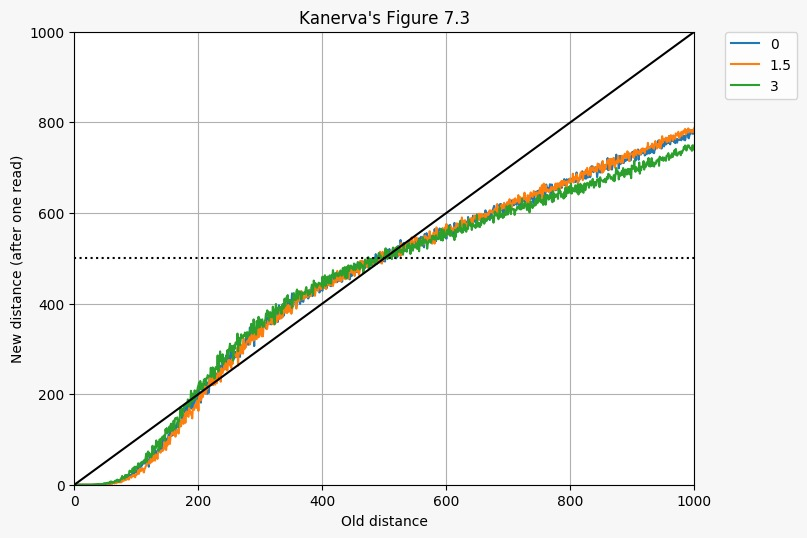
\includegraphics[width=\linewidth]{./images02/new-images/z_0_15_3.jpg}
  \caption{z  0  15  3.jpg}
  \label{fig:boat1}
\end{figure}

Figure \ref{fig:boat1} shows a boat.

/images02/new-images/



\begin{figure}
  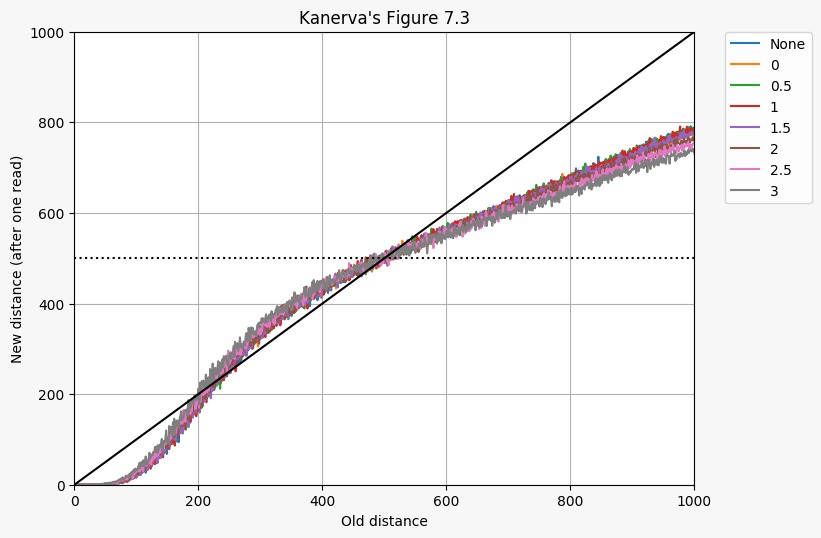
\includegraphics[width=\linewidth]{./images02/new-images/z_all.jpg}
  \caption{z  all.jpg}
  \label{fig:boat1}
\end{figure}








\begin{figure}
  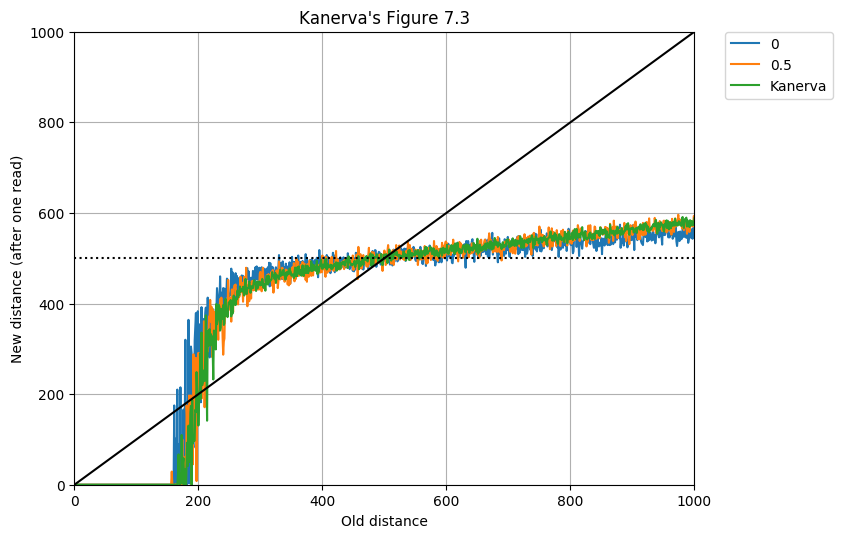
\includegraphics[width=\linewidth]{./images02/new-images/iter_z_0_05_1.png}
  \caption{iter z  0  0.5 1.png}
  \label{fig:boat1}
\end{figure}




\begin{figure}
  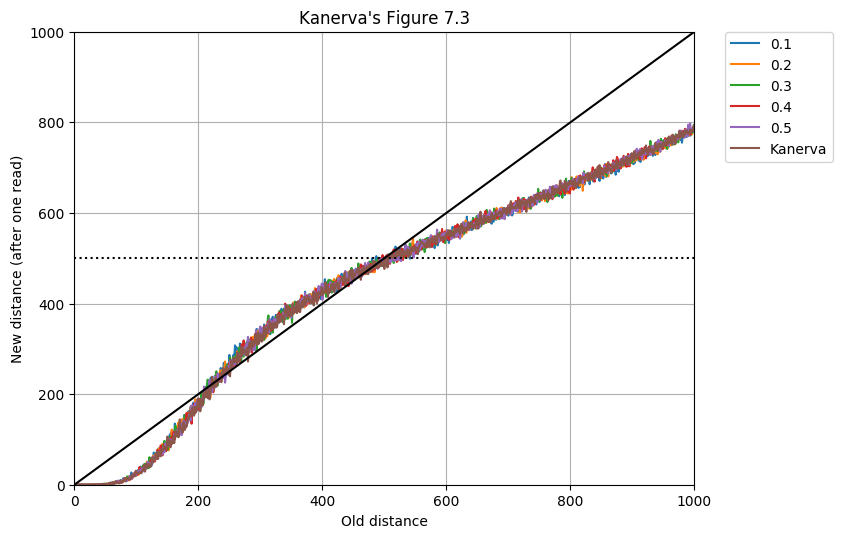
\includegraphics[width=\linewidth]{./images02/new-images/iter_z_01-05.png}
  \caption{iter z 01-05.png}
  \label{fig:boat1}
\end{figure}



\begin{figure}
  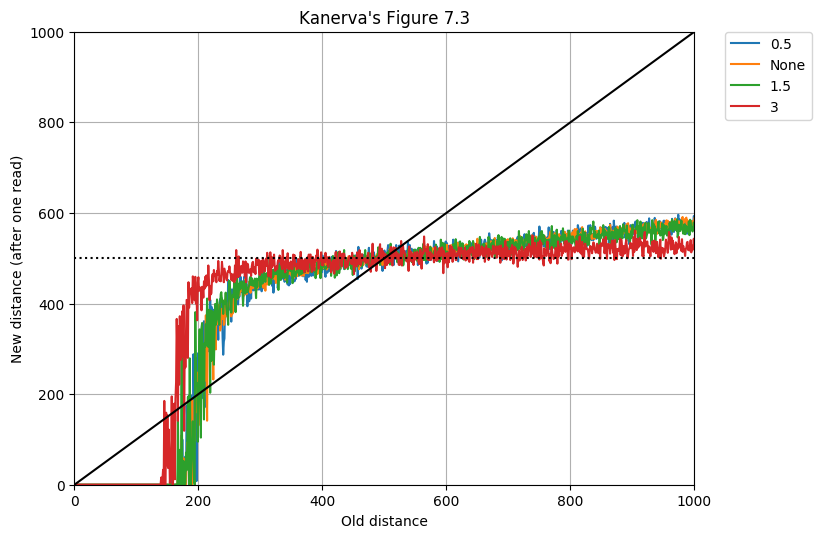
\includegraphics[width=\linewidth]{./images02/new-images/iter_z_05_1_15_3.png}
  \caption{iter z  0.5 1 1.5 3.png}
  \label{fig:boat1}
\end{figure}



\begin{figure}
  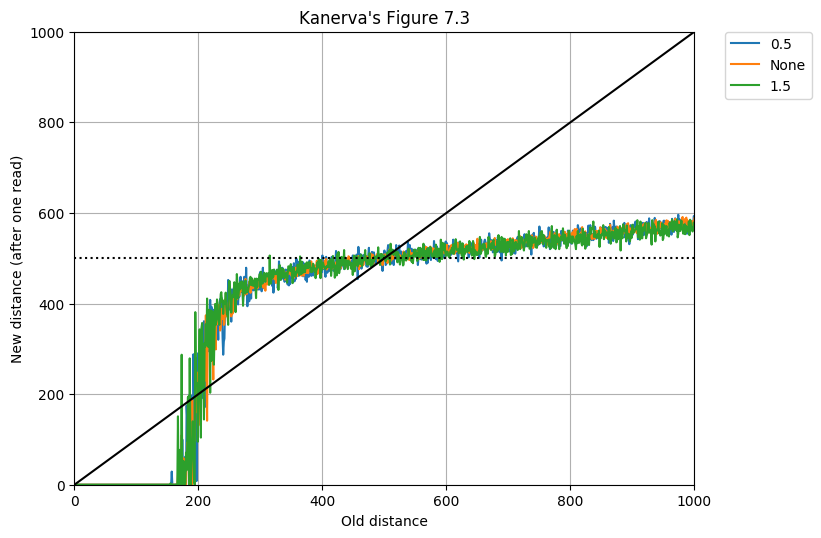
\includegraphics[width=\linewidth]{./images02/new-images/iter_z_05_1_15.png}
  \caption{iter $z\in \{0.5, 1, 1.5\}$ }
  \label{fig:boat1}
\end{figure}



\begin{figure}
  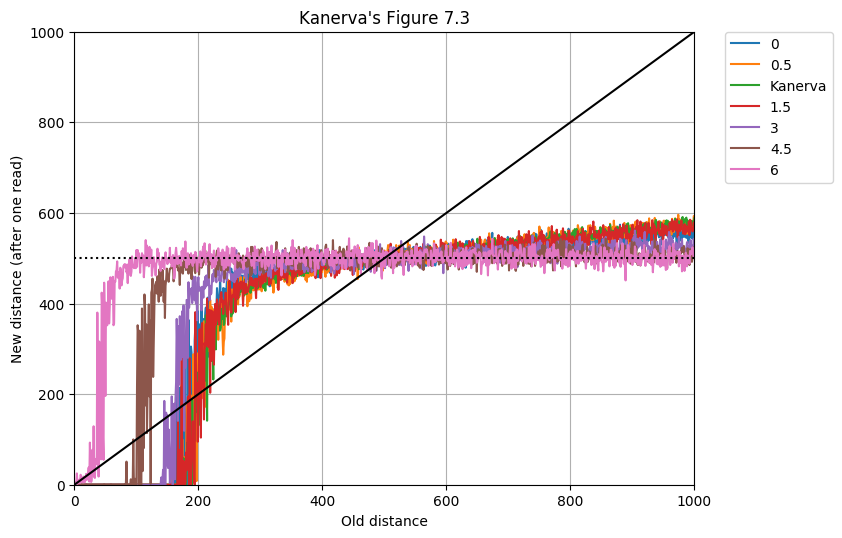
\includegraphics[width=\linewidth]{./images02/new-images/iter_z_all_2.png}
  \caption{iter z all 2.png}
  \label{fig:boat1}
\end{figure}



\begin{figure}
  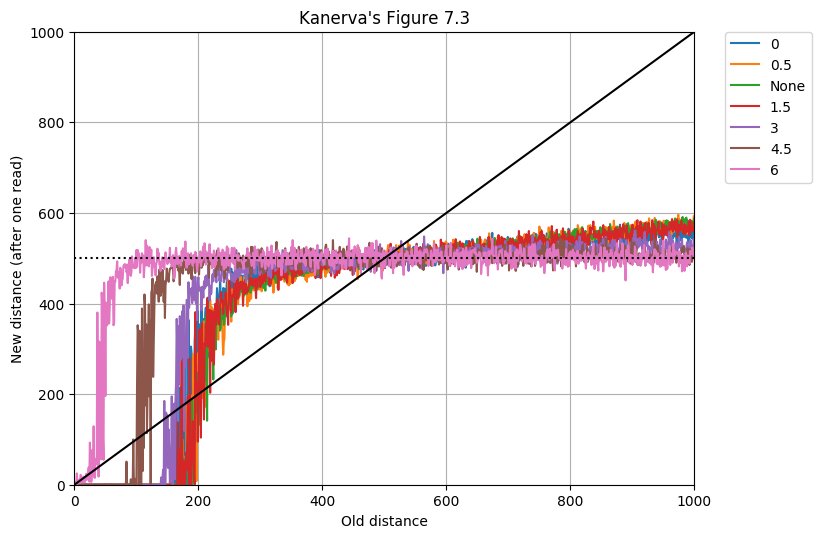
\includegraphics[width=\linewidth]{./images02/new-images/iter_z_all.png}
  \caption{iter z all.png}
  \label{fig:boat1}
\end{figure}





\begin{figure}
  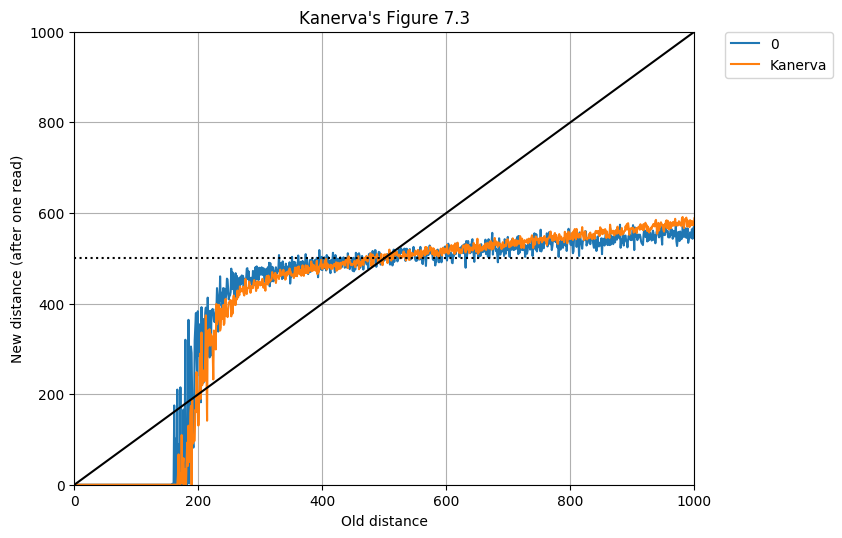
\includegraphics[width=\linewidth]{./images02/new-images/z_0_1.png}
  \caption{z 0 1.png}
  \label{fig:boat1}
\end{figure}



\begin{figure}
  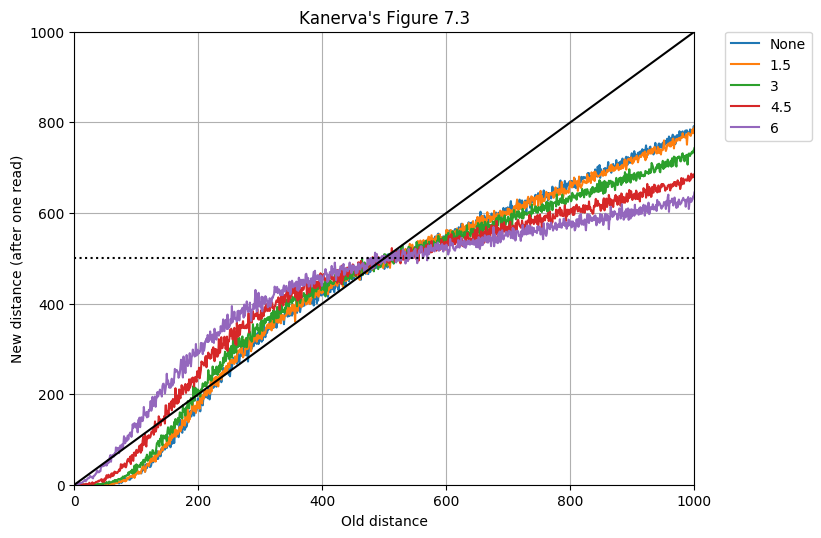
\includegraphics[width=\linewidth]{./images02/new-images/z_1_15_3_45_6.png}
  \caption{z 1 1.5 3 4.5 6.png}
  \label{fig:boat1}
\end{figure}



\begin{figure}
  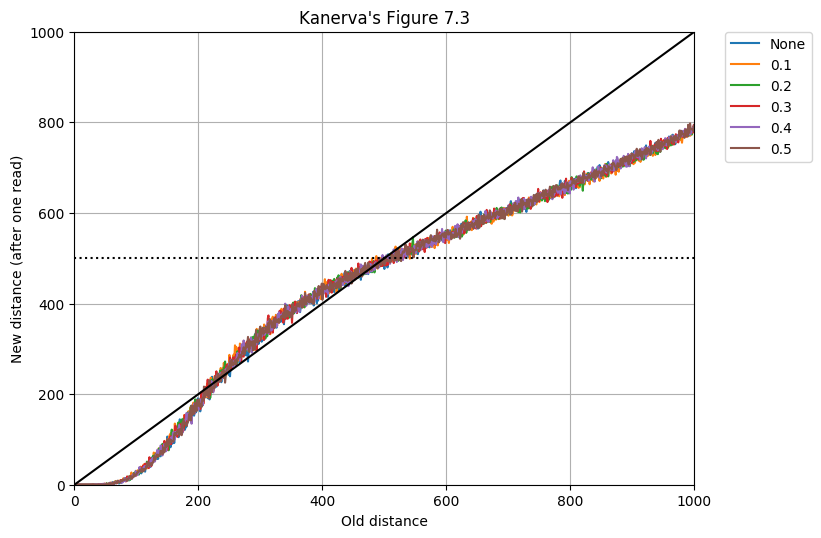
\includegraphics[width=\linewidth]{./images02/new-images/z_01-05.png}
  \caption{z 01 - 05.png}
  \label{fig:boat1}
\end{figure}



\begin{figure}
  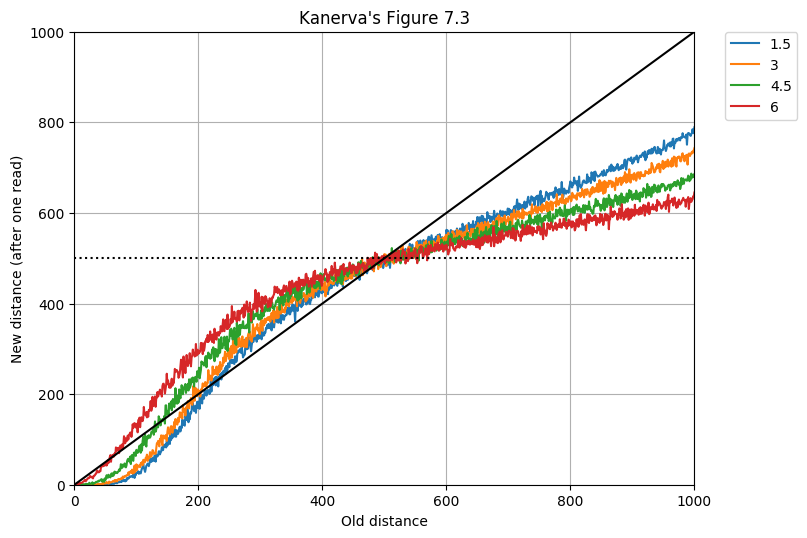
\includegraphics[width=\linewidth]{./images02/new-images/z_15_3_45_6.png}
  \caption{z 1.5 3 4.5 6.png}
  \label{fig:boat1}
\end{figure}



\begin{figure}
  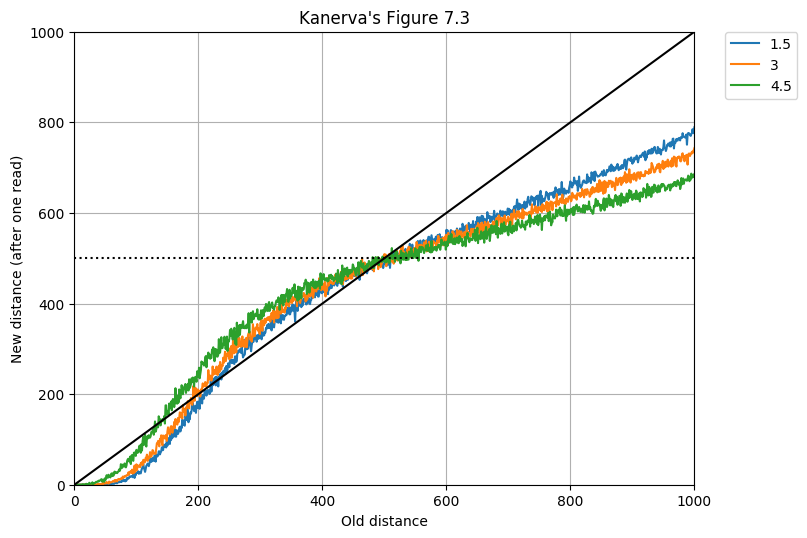
\includegraphics[width=\linewidth]{./images02/new-images/z_15_3_45.png}
  \caption{z 1.5 3 4.5.png}
  \label{fig:boat1}
\end{figure}


faltando as imagens do google doc...
\section{Critical Distance}

\begin{figure}[h!]
\centering

\subfloat[]{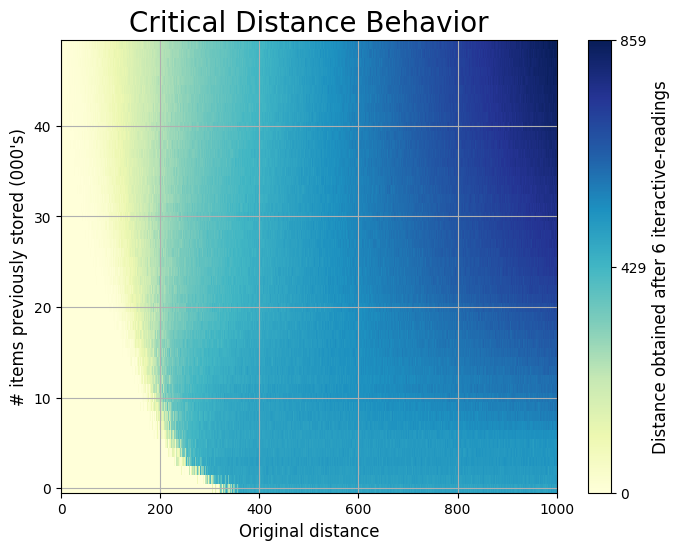
\includegraphics[width=3.1in]{./images02/new-images/kanerva-read.png}}

\subfloat[]{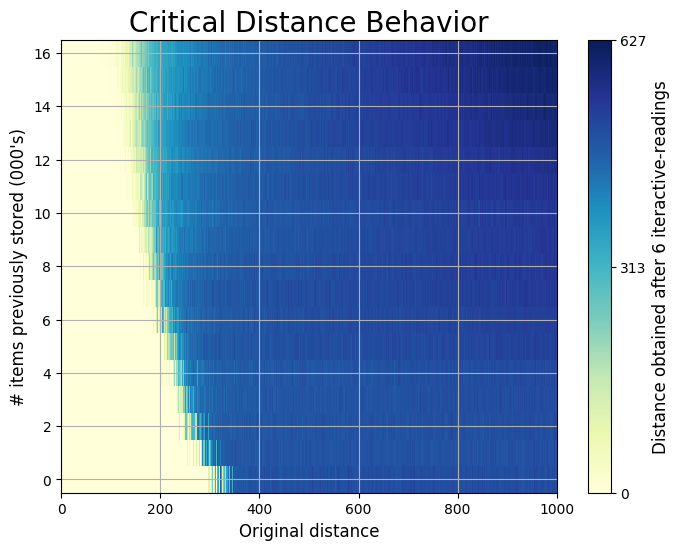
\includegraphics[width=3.1in]{./images02/new-images/chada-read_z_0.png}}

\caption{The critical distance behavior, as the memory is written with items.  The colors of this heatmap display the hamming distance to the item being read as a function of the distance from that item and the numbers of items registered in memory.  In the $x$-axis, the distance from the item being read is displayed. In the $y$-axis, we display the read operation's behavior as the number of items registered in the memory grows.  In (a), we have Kanerva's original model; whereas (b) displays Chada's read.}
\label{fig:crit-dist-10k-writes}

\end{figure}



\section{Speculations on the use of Information Theory}

\begin{figure}
  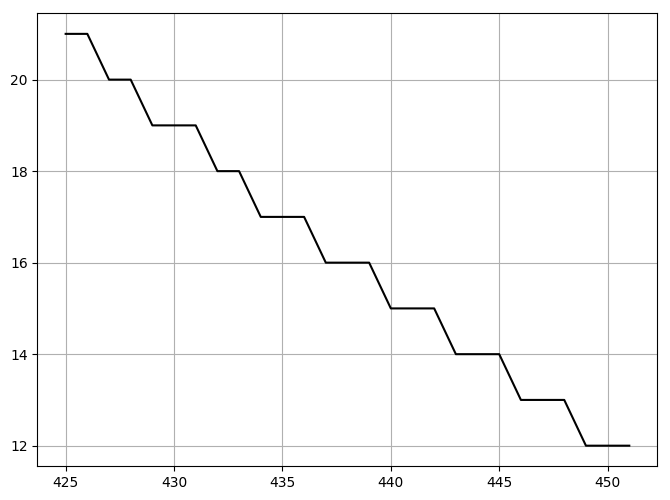
\includegraphics[width=\linewidth]{./images02/new-images/information_decay.png}
  \caption{information decay 4.png}
  \label{fig:boat1}
\end{figure}




\subsection{A subsection}

More text.

\end{document}
